%!TEX TS-program = xelatex
% !TEX root = ../thesis.tex
% Do not delete; used to set build system

\chapter{Online supplement for ``Template-based estimation of genome-wide nucleosome positioning via distributed HMC''}

\section{Algorithmic details of inference}

\subsection{Distributed HMC sampler}
\label{sec:mcmc}

Recall that the model specified in Section 2 is:
\begin{align}
 \label{eq:observation_model}
  y_k|\lambda_k         & \sim \hbox{Poisson } (\lambda_k) \\
 \label{eq:linear_model}
  \lambda_{(N\times 1)} & \equiv X_{(N\times (N - \ell_0))} ~ \beta_{((N - \ell_0)\times 1)}, \\
\nonumber & \quad \beta_k>0 \hbox{ for } k=\lfloor \ell_0 / 2 \rfloor + 1 \dots N - \lfloor \ell_0 / 2 \rfloor \\
\label{eq:positioning_model}
  \log \beta_k        & \sim \hbox{Normal } (\mu_{s_k},\sigma^2_{s_k})
\end{align}
given a segmentation function $\fnDef{s}{\range{1}{N}}{\range{1}{S}}$, which maps the $N$ base pair locations to $S$ regions in which coefficients $\beta_k$ can be assumed to be identically distributed.
$X$ specifies the contribution of a nucleosome positioned at base pair $k$ to the expected number of reads at base pair $m$ due to digestion variability, and $s(k)$ is denoted as $s_k$ for compactness.
This specification is completed with independent priors on each $(\mu_s, \sigma^2_s)$:
\begin{align}
\sigma^2_{s} &\sim \mathrm{InvGamma}(\alpha_0, \gamma_0) \ , \\
\mu_{s} | \sigma^2_{s} &\sim N(\mu_0, \frac{\sigma^2_{s}}{n_{s} \tau_0}) \ ,
\end{align}
where $n_{s}$ is the length of segment $s$.

Our MCMC sampler alternates between two conditional updates:
\begin{enumerate}
 \item Draw $(\bm \mu^{(r)}, \bm \sigma^{2\,(r)}) | \bm \beta^{(r-1)}$ directly, then
 \item Update $\bm \beta^{(r)} | (\bm \mu^{(r)}, \bm \sigma^{2\,(r)})$ via a distributed HMC step.
\end{enumerate}
The former is a standard conjugate draw, while the latter is done via a distributed version of the standard Hamiltonian Monte Carlo (HMC) routine.

\subsubsection{Hyperparameter updates}

In detail, step 1 consists of the following draws for each $(\mu_s, \sigma^2_s)$, defining $\bm \theta = \log \bm \beta$:
\begin{align}
 \sigma_s^{2\,(r)} | \bm \beta^{(r-1)} &\sim InvGamma{\bigg(}\frac{n_s}{2} + \alpha_0,
  \, \frac{1}{2} \sum_{k:s_k = s} (\theta_k^{(r-1)} - \bar{\theta}_s^{(r-1)})^2  \\
\nonumber
  & + \frac{\tau_0 n_s}{2 (1 + \tau_0)} (\bar{\theta}_s^{(r-1)} - \mu_0)^2
  + \gamma_0 {\bigg)} \ , \\
 \mu_s^{(r)} | \sigma_s^{2\,(r)}, \bm \beta^{(r-1)} &\sim N\left( \frac{\bar{\theta}_s^{(r-1)} + \tau_0 \mu_0}{1 + \tau_0}, \frac{\sigma_s^{2\,(r)}}{n_s (1 + \tau_0)} \right) \ ,
\end{align}
where $\bar{\theta}_s^{(r-1)} = \frac{1}{n_s} \sum_{k : s_k = s} \theta_k^{(r-1)}$.
These are standard conjugate updates and have computational and memory complexity $O(N)$.

\subsubsection{Distributed HMC update for \texorpdfstring{$\bm \beta$}{beta}}
\label{sec:distributedHMC}

The draws in step 2 proceed in two stages, using two partitions of $\bm \beta$.
The first starts at the beginning of $\bm \beta$ and proceeds forward with subvectors of length at most $B$ separated by $2w$, yielding
\begin{align}
D_1 &= \bm \beta_{[1 : B]}, \bm \beta_{[B + 2w + 1 : 2B + 2w]}, \ldots, \bm \beta_{[n_b (B + 2w) + 1 : N]} \ , \\
D_2 &= \bm \beta_{[B/2 + 1 : 3B/2]}, \bm \beta_{[3B/2 + 2w + 1 : 5B/2 + 2w]}, \ldots, \bm \beta_{[n_b (B + 2w) B/2 + 1 : N]} \ .
\end{align}
The subvectors within each partition are conditionally-independent given the $(\bm \mu, \bm \sigma^2)$ and the entries of $\bm \beta$ separating them.
Hence, we can update them in parallel across multiple processors.
The basic structure of these updates follows Algorithm \ref{alg:master}.
%
\begin{algorithm}%[ht]
 \hspace{-8pt} \textbf{Distributed HMC update}\\

 \tcc{Send conditioning information}
 Broadcast $\bm \mu^{(t-1)}$, and $\bm \sigma^{2\,(t-1)}$ to all workers \;

 \For{offset \KwTo (0, $B/2$)} {
 \tcc{Send first round of jobs to workers}
 \For{w \KwTo \Range{min(nWorkers, nBlocks)}}{
   $start = \max(0, (w - 1)(B + 2w) - 2w + \mbox{offset}) + 1$\;
   $end = \min(N, w(B + 2w) + 2w + \mbox{offset})$\;
   Send $\bm \theta[start:end] $ to worker process w with work tag attached \;
 }
 \If{ len(startVec) $<$ nWorkers }{
   Pause remaining workers \;
 }

 \tcc{Collect results}
 Set \textit{nComplete} = 0, \textit{nStarted} = min(nWorkers, nBlocks) \\
 \While{nComplete $<$ nBlocks } {
   Receive result $\bm \theta[start:end]$ from arbitrary worker with tag $b_1$ \;
   Incorporate result into working copy of $\bm \theta^{(t)}$ \;
   \textit{nComplete}++ \;
   \If{nStarted $<$ nBlocks} {
     \tcc{Send additional jobs as needed}
     $w = nStarted + 1$\;
     $start = \max(0, (w - 1)(B + 2w) - 2w + \mbox{offset}) + 1$\;
     $end = \min(N, w(B + 2w) + 2w + \mbox{offset})$\;
     Send $\bm \theta[start:end] $ to last completed worker process with work tag attached\;
     \textit{nStarted}++\;
   }
 }
}

 \caption{Distributed HMC update \label{alg:master}}
\end{algorithm}

The individual, worker-level HMC updates are done on $\bm \theta = \log \bm \beta$ and follow the standard leapfrog-based HMC procedure outlined in \citet{Neal2010}.
To compute these HMC updates, we require the log-posterior density of each subvector of $\bm \theta$ and its gradient.
First, define $\bm \lambda = X \bm \beta$, $\bm m = (\mu_{s_k} \mbox{ for } k = 1, \ldots, N)^\top$, and $\bm v = (\sigma^2_{s_k} \mbox{ for } k = 1, \ldots, N)^\top$.
Also, for vectors of equal dimension, let $/$ denote entrywise division and $**$ denote entrywise powers.
Then,
\begin{align}
\log p(\bm \theta | \bm \mu, \bm \sigma^2) &= -\bm 1^\top X \bm \beta + \sum_k y_k \log \left( \bm x_k^T \bm \beta \right) \\
\nonumber
&\phantom{=} - \frac{1}{2} \sum_k \frac{(\theta_k - \mu_{s_k})^2}{\sigma^2_{s_k}} + \mathrm{const} \ , \\
\nabla_{\bm \theta} \log p(\bm \theta | \bm \mu, \bm \sigma^2) &= -\diag{\bm \beta} X^\top (\bm 1 - \bm y / \bm \lambda) - (\bm \theta - \bm m) / \bm v \ , \\
\nabla_{\bm \theta} \nabla_{\bm \theta^\top} \log p(\bm \theta | \bm \mu, \bm \sigma^2) &= -\diag{\bm \beta} X'WX \diag{\bm \beta} \\
\nonumber
&\phantom{=} - \diag{\bm \beta} X' (\bm 1 - \bm y
/ \bm \lambda) - \diag{\bm 1 / \bm \sigma^2} \label{eq:hessian} \ ,
\end{align}
where $W = \diag{\bm y / \bm \lambda\mbox{**}2}$.
Due to the convolution structure of $X$, all matrix-vector products involving $X$ and $X^\top$ can be reduced to convolutions of vectors with the template vector $\bm t$.
This also enables efficient computation of the Hessian's diagonal, as
\begin{align}
\bm \lambda &= X \bm \beta = (\bm 0_{\lfloor \ell_0 / 2 \rfloor}^\top \; \bm \beta^\top \; \bm 0_{\lfloor \ell_0 / 2 \rfloor}^\top)^\top \convolution \bm t \\
X^\top (\bm 1 - y / \bm \lambda) &= (\bm 1 - y / \bm \lambda) \convolution \bm t \ , \\
\diag{X'WX} &= (\bm y / \bm \lambda\mbox{**}2) \convolution \bm t\mbox{**}2 \ .
\end{align}
%
This reduces the computational complexity of these evaluations to $O(B \log B)$ for each update of each subvector of $\bm \beta$.
Our block-level HMC steps are detailed in Algorithm \ref{alg:hmc}.
%
\begin{algorithm}%[ht]

 \KwData{Trajectory length $L$, $\bm \mu$, $\bm \sigma^2$, $\bm \theta[start:end]$, $\epsilon{\min}$, $\epsilon_{\max}$, block start $b$, template $\bm t$, chromosome length $N$}
 \tcc{Subset $\bm \theta[start:end]$ to B-length subvector to update and buffers}
 $\bm{\tilde \theta} = \bm \theta[ b : \min(b + B - 1, N)]$\;
 $\bm{\tilde \theta}_0 = \bm{\tilde \theta}$;
 $\bm{\underline \theta} = (\bm \theta[start:b], \bm \theta[\min(b + B - 1, N):end])$\;
 Draw step size $\epsilon \sim \Unif[\epsilon_{\min}, \epsilon_{\max}]$\;
 \tcc{Optionally estimate mass matrix from Hessian; default is identity}
 \If{Estimating mass matrix}{
  Maximize log conditional posterior to obtain $\bm \hat{\theta}$\;
  $M = -\nabla_{\bm{\tilde \theta}} \nabla_{\bm{\hat \theta}^\top} \log p(\bm{\hat \theta} | \bm \mu, \bm \sigma^2, \bm{\underline \theta} )$\;
  \If{Using diagonal mass matrix} {
   $M = \diag{M}$\;
  }
 }
 \Else{
  $M = I_{end - start}$\;
 }
 \tcc{Draw momentum}
 Draw $\bm p \sim N(\bm 0, M)$\;
 $\bm p_0 = \bm p$\;
 \tcc{Run leapfrog integration}
 $\bm p += \epsilon \nabla_{\bm{\tilde \theta}} \log p(\bm{\tilde \theta} | \bm \mu, \bm \sigma^2, \bm{\underline \theta}) / 2$\;
 \For{i \KwTo \Range{$L$}}{
  $\bm{\tilde \theta} += \epsilon M^{-1} p$\;
  \If{$i < L - 1$}{
   $\bm p += \epsilon \nabla_{\bm{\tilde \theta}} \log p(\bm{\tilde \theta} | \bm \mu, \bm \sigma^2, \bm{\underline \theta})$\;
  }
 }
 $\bm p += \epsilon \nabla_{\bm{\tilde \theta}} \log p(\bm{\tilde \theta} | \bm \mu, \bm \sigma^2, \bm{\underline \theta}) / 2$\;
 \tcc{Metropolis-Hastings step to correct for integration errors}
 $\log r = \log p(\bm{\tilde \theta} | \bm \mu, \bm \sigma^2, \bm{\underline \theta}) - \log p(\bm{\tilde \theta}_0 | \bm \mu, \bm \sigma^2, \bm{\underline \theta}) - 1/2( \bm p^\top M^{-1} \bm p - \bm p_0^\top M^{-1} \bm p_0)$\;
Draw $u ~ \Unif[0,1]$\;
\If{$u \leq r$} {
\Return{$(\bm{\tilde \theta}, 1)$} \tcc*{Accept update}
}
\Else {
\Return{$(\bm{\tilde \theta}_0, 0)$} \tcc*{Reject update}
}
 \caption{Worker-level HMC update \label{alg:hmc}}
\end{algorithm}
%
In practice, we fix $\epsilon_{\min} = 0.001$, $\epsilon_{\max} = 0.1$, and $L = 100$.
We also use a fixed diagonal mass matrix, although the algorithm can accommodate estimating it at every iteration if needed.
However, to maintain the $O(B \log B)$ scaling of our algorithm's complexity with block size, $M$ must remain diagonal.
If non-diagonal $M$ is used and/or estimated, our HMC update instead scales as $O(B^2)$.
In either case, the overall algorithm scales $O(N)$ for given a fixed block size $B$.
%
Memory requirements are $O(N)$ for the master process running the hyperparameter draws and coordinating the distributed HMC updates.
Each worker process requires $O(B \log B)$ memory to run the distributed HMC updates for diagonal $M$, while using a non-diagonal mass matrix $M$ requires $O(B^2)$ memory per worker.


%%%%%%%%%%%%%%%%%%%%%%%%%%%%%%%%%%%%%%%%%%%%%%%%%%%%%%%%%%%%%%%%%%%%%%%%%%%%%%%%
\subsection{Approximate EM algorithm}
\label{sec:approxem}

We develop an approximate EM algorithm, based on a Gaussian approximation of the conditional posterior of $\bm \theta$, as to obtain starting values for the MCMC sampler given in \ref{sec:mcmc}.
It provides a high-quality initialization for $\bm \beta$, $\bm \mu$, and $\bm \sigma^2$.
Simpler initializations are possible, but obtaining high-quality initial estimates can greatly reduce the number of MCMC iterations required for reliable inferences.

\subsubsection{Choice initial estimator}
\label{sec:objective}

We use $\hat \theta_k = E \left[ \theta_k | \bm y, \hat \mu_{s_k}, \hat \sigma^2_{s_k} \right]$ as an initial point estimate of $\theta_k$.
The distributed HMC sampler presented in Section \ref{sec:mcmc} yields information on the complete marginal posterior of $\bm \theta$ via simulation but, given the scale of this problem, an optimization-based approach is useful as a fast initialization method.
The approximate EM algorithm described in Section \ref{sec:approximate_em} provides both approximate marginal MAP estimates of the parameters $\bm \mu$ and $\bm \sigma^2$ and estimates of the target conditional expectations $\hat \theta_k$.

\subsubsection{Approximate EM algorithm via Laplace approximation}
\label{sec:approximate_em}

We implement an approximate EM algorithm to provide initial estimates of $(\bm \theta, \bm \mu, \bm \sigma)$.
In the E-step, we build an approximation of the conditional posterior of ${\bm \theta}$ given $(\bm y, \hat {\bm\mu}, \hat{\bm\sigma}^2)$ to estimate the $Q$ function, detailed below.
The M-step updates the estimates of $\bm \mu$ and $\bm \sigma^2$ toward the marginal posterior mode of $p(\bm \mu, \bm \sigma^2 | \bm y)$.

\paragraph{Approximate E-step}
%
In the E-step, the objective is to compute 
\begin{equation} 
  Q_t(\bm \mu, \bm \sigma^2) = E \left[ \log p(\bm \theta, \bm \mu, \bm \sigma^2 | \bm y ) | \bm y, \bm \mu^{(r-1)}, \bm \sigma^{2\,(r-1)} \right].
\end{equation}
%
The log joint posterior for $(\bm \mu, \bm \sigma^2, \bm \theta)$ is given by
\begin{eqnarray}\label{eq:logPosterior}
 \log p(\bm \theta, \bm \mu, \bm \sigma^2 | \bm y, \bm s, \tau_0) &=& -\sum_k
\bm x_k^T \beta_k + \sum_k y_k \log \left( \bm x_k^T \beta_k \right)  \\
 \nonumber && - \frac{1}{2} \sum_k \log \sigma^2_{s_k} -
  \frac{1}{2} \sum_k \frac{(\theta_k - \mu_{s_k})^2}{\sigma^2_{s_k}} \\
 \nonumber && - \frac{1}{2} \sum_s \log \left( \frac{\sigma^2_{s}}{n_{s} \tau_0}
  \right) - \frac{1}{2} \sum_s \frac{(\mu_s - \mu_0)^2}{\sigma^2_{s} / n_{s} \tau_0} \\
  \nonumber && - \sum_s \log \sigma^2_s + \mathrm{const}.
\end{eqnarray}
%
Thus, we can write the relevant portion of the expected log conditional
posterior for $\bm \theta$ given $\{\mu_{s_k}, \sigma^2_{s_k}\}$ as
\begin{eqnarray}
 Q_t(\bm \mu, \bm \sigma^2) &=& - \frac{1}{2} \sum_k \log \sigma^2_{s_k} -
  \frac{1}{2} \sum_k \frac{(\hat{\theta}_k - \mu_{s_k})^2}{\sigma^2_{s_k}}
 - \frac{1}{2} \sum_k \frac{\hat{V}_k}{\sigma^2_{s_k}} \\
 \nonumber && - \frac{1}{2} \sum_s \log \left( \frac{\sigma^2_{s}}{n_{s} \tau_0}
  \right) - \frac{1}{2} \sum_s \frac{(\mu_s - \mu_0)^2}{\sigma^2_{s} / n_{s} \tau_0}
 - \sum_s \log \sigma^2_s.
\end{eqnarray}
where $\hat{\theta}_k = E[ \theta_k | \bm \mu_{(t-1)}, \bm \sigma^2_{(t-1)} ]$
and $\hat{V}_k = \Var [ \theta_k | \bm \mu_{(t-1)}, \bm \sigma^2_{(t-1)} ]$. 

While the conditional posterior $p(\bm \theta | \bm y, \bm \mu, \bm \sigma^2 )$ is available in close form,  the necessary  expectations $\hat{\theta}_k$ and variances $\hat V_k$ are not.
However, under the proposed log-Normal/Poisson model structure, the univariate conditional posteriors of $\theta_k$ given $\{\mu_{s_k}, \sigma^2_{s_k}\}$ are unimodal, log-concave, nearly symmetric, and have tails that go to zero as $\exp(-c \theta_k^2)$. 
Thus, these conditional posteriors are nearly Gaussian and a Laplace approximation is appropriate. 

To compute the Laplace approximation, we first find the posterior mode of
$\theta_k$ given $(\bm \mu^{(r-1)}, \bm \sigma^{2\,(r-1)})$. This amounts to
maximizing
\begin{equation}\label{eq:gFunction}
 g(\bm \theta) = -\sum_k \bm x_k^T \beta_k +
\sum_k y_k \log \left( \bm x_k^T \beta_k \right) -
\frac{1}{2} \sum_k \frac{(\theta_k - \mu_{s_k})^2}{\sigma^2_{s_k}}
\end{equation}
with respect to $\bm \theta$.
This mode is not available in closed form, but the given objective function is concave and has a continuous gradient, so numerical optimization is feasible.
%\footnote{To preserve the vector notation throughout the gradient and the Hessian calculations, we use the two following chain rules: $\frac{dg}{d\theta} = \frac{dg}{d\beta} \cdot \frac{d\beta}{d\theta} = \frac{dg}{d\beta} \cdot \beta$ and $\frac{d^2 g}{d\theta^2} = \frac{dg}{d\beta} \cdot \frac{d^2 \beta}{d\theta^2} + \frac{d^2 g}{d\beta^2} \cdot (\frac{d \beta}{d\theta})^2 = \frac{dg}{d\beta} \cdot \beta + \frac{d^2 g}{d\beta^2} \cdot \beta^2$} 

%
The Laplace approximation then consists of substituting a Gaussian distribution with mean $\bm \hat{\theta}_t$ equal to the mode of $g$, and variance $\hat{V}_k = -\diag{H^{-1}}_k$ for the conditional posterior $p(\theta_k | \bm y, \mu_{s_k}, \sigma^2_{s_k} )$.

\paragraph{M-step}
%
The M-step consists of maximizing $Q_t(\bm \mu, \bm \sigma^2)$ with respect to $\mu_{s_k}$ and $\sigma^2_{s_k}$.
We obtain two simple closed-form solutions, summarized in Equations \ref{eq:mstep-mu} and \ref{eq:mstep-sigmasq}:
\begin{eqnarray} \label{eq:mstep-mu}
\hat{\mu}_{s} &=& \frac{1}{1 + \tau_0} \Big(\frac{1}{n_s}
 \sum_{k:s_k = s} \hat{\theta}_k \Big) +
 \frac{\tau_0}{1 + \tau_0} \mu_0 \\ \label{eq:mstep-sigmasq}
\hat{\sigma}^2_{s} &=& \frac{\frac{1}{n_s} \sum_{k:s_k = s}
 (\hat{\theta}_k - \hat{\mu}_{s})^2
 + \frac{1}{n_s} \sum_{k:s_k = s} \hat{V}_k +
 \tau_0 (\hat{\mu}_s - \mu_0)^2}{1+\tau_0 + 2 / n_s}
\end{eqnarray}

The term $\hat{V}_k$ differentiates the M-step update of $\sigma_s$ from the update obtained from joint maximization of the log-posterior.
The joint mode of this log-posterior is reached at $\bm \sigma^2 = \bm 0$ and $\theta_k = \mu_{s_k} \, \forall k$, as these values would allow the joint log-posterior density to increase without bound.
Algorithmically, the $\hat{V}_k$ term introduced by the EM algorithm prevents $\hat{\sigma}^2$ from collapsing to $0$, providing non-degenerate inferences.

% AWB: Perhaps add pointer to new algorithm without blocked E-step for overview of process; seems less necessary at this point

\subsubsection{Distributed approximate E-step}
\label{sec:parallelization}

We use the conditional independence structure of $\bm \beta$ given $(\bm \mu, \bm \sigma^2)$ and partitions discussed in Section \ref{sec:distributedHMC} to distribute our approximate E-step across multiple processors.
Given each partition of $\bm \theta$, we update the Laplace approximations in parallel, by finding the mode of the conditional posterior subvector-by-subvector.
The overall algorithm is blockwise coordinate ascent within each approximate E-step, with each E-step consisting of iterative maximization of $\log p(\bm \theta | \bm y, \bm \mu, \bm \sigma^2 )$ using different subsets of $\bm \theta$ (corresponding to different blocks) in each iteration.
This converges to the maximum of $g(\bm \theta)$ given $\bm \mu^{(r-1)}$ and $\bm \sigma^{2\,(r-1)}$.

The approximate E-step considers each block in each of the four configurations, during one iteration. 
More details are give in Section \ref{sec:mpi}.
Within each block $m_1:m_2$, we maximize $\log p(\bm \theta_{m_1:m_2} | \bm y, \bm \mu, \bm \sigma^2, \bm \theta_{-(m_1:m_2)} )$ numerically via L-BFGS-B or a truncated Newton algorithm \citep{lbfgsb1997, Nash2000}; the latter is typically more efficient in this application.
We carry out this maximization directly, avoiding the data augmentation typically used in additive Poisson models of this type \citep[e.g.,][]{VanDykEtAl2006}. 
Such data augmentation would require storing and computing at least $(2w+1)N$ additional variables, provide slower convergence, and slow the overall computation substantially.
By controlling the size of the blocks, we can keep the scale of each optimization problem small enough that direct numerical maximization of these conditional posteriors is not a limiting factor for the algorithm (less than 100ms, typically).

We compute the Hessian of the conditional log-posterior $\log p(\bm \theta | \bm y, \bm \mu, \bm \sigma^2 )$ after each complete scan through the partitions, completing the approximate E-step and providing the information necessary for our M-step.
The Hessian is sparse, but its inversion is computationally-intensive even with modern sparse-matrix solvers.
Thus, we typically use a diagonal approximation to the Hessian.
The diagonal approximation works well in our setting, even though one would expect the strong local dependence generated by the digestion matrix to produce a Hessian with large off-diagonal elements.
However, due to the use of exchangeable local regularization, the Hessian is typically diagonally-dominant.
The diagonal approximation is quite accurate; we observed few differences to 2-3 significant digits in comparisons of the estimated Hessian and its inverse on small portions of the genome (single ORFs with promoters, approximately 1,000 to 10,000bp in length).
%
We lay out the overall structure of this approximate EM algorithm in Algorithm \ref{alg:deconvolve}.

\begin{algorithm}%[ht]
\hspace{-8pt} \textbf{Outline of Approximate EM Algorithm} \\
 \While{not converged} {
  \tcc{E-step}
	\For{Partition \KwTo $(D_1, D_2)$}{
  Update $\hat{\bm \theta}$ via numerical maximization of $g(\bm \theta)$ within each subvector
	}
% AWB: Added nested for-loop with blockwise maximizations and scan
  Approximate $\Var \left[ \theta_k | \bm y, \mu_{s_k}, \sigma^2_{s_k}
    \right]$ by inverting Hessian of $p(\bm \theta | \bm y, \bm \mu, \bm
    \sigma^2 )$
  
  \tcc{M-step}
  Update $\bm \mu$ and $\bm \sigma^2$ as maximizers of $E \left[ p(\bm \theta,
    \bm \mu, \bm \sigma^2 | \bm y, \bm s, \tau_0) | \bm \mu_{(t-1)}, \bm
    \sigma^2_{(t-1)}, \bm s, \bm \tau_0 \right]$
 }
 \caption{Approximate EM Algorithm \label{alg:deconvolve}}
\end{algorithm}

\subsubsection{Algorithmic details}
\label{sec:mpi}

The algorithm outlined in Section \ref{sec:approximate_em} can be implemented on distributed systems with MPI, using the same techniques as the MCMC algorithm presented in Section \ref{sec:mcmc}.
Due to the use of a quasi-Newton optimization algorithm within each worker's approximate E-step, its computational complexity scales $O(B^2)$ for each such update.
However, it scales $O(N)$ in the length of genome given a fixed block size $B$.
Memory requirements are $O(N)$ for the master process running the M-step and coordinating the approximate E-step and $O(B^2)$ (independent of $N$) for the worker processes running the approximate E-step updates.
We lay out the details of this parallel approximate E-step in Algorithm \ref{alg:parallel}.

\begin{algorithm}%[ht]
 \hspace{-8pt} \textbf{Parallel Implementation of Approximate E-Step}\\
 \tcc{Send conditioning information}
 Broadcast $\bm \mu^{(t-1)}$, and $\bm \sigma^{2\,(t-1)}$ to all workers \;

 \For{offset \KwTo (0, $B/2$)} {
 \tcc{Send first round of jobs to workers}
 \For{w \KwTo \Range{min(nWorkers, nBlocks)}}{
   $start = \max(0, (w - 1)(B + 2w) - 2w + \mbox{offset}) + 1$\;
   $end = \min(N, w(B + 2w) + 2w + \mbox{offset})$\;
   Send $\bm \theta[start:end] $ to worker process w with work tag attached \;
 }
 \If{ len(startVec) $<$ nWorkers }{
   Pause remaining workers \;
 }

 \tcc{Collect results}
 Set \textit{nComplete} = 0, \textit{nStarted} = min(nWorkers, nBlocks) \\
 \While{nComplete $<$ nBlocks } {
   Receive result $\bm \theta[start:end]$ from arbitrary worker with tag $b_1$ \;
   Incorporate result into working copy of $\bm \theta^{(t)}$ \;
   \textit{nComplete}++ \;
   \If{nStarted $<$ nBlocks} {
     \tcc{Send additional jobs as needed}
     $w = nStarted + 1$\;
     $start = \max(0, (w - 1)(B + 2w) - 2w + \mbox{offset}) + 1$\;
     $end = \min(N, w(B + 2w) + 2w + \mbox{offset})$\;
     Send $\bm \theta[start:end] $ to last completed worker process with work tag attached\;
     \textit{nStarted}++\;
   }
 }
 }

 \tcc{Compute approximate variance, if needed}
 Compute approximate $\Var \left[ \theta_k | \bm y, \mu_{s_k}, \sigma^2_{s_k}  \right]$ using sparse Cholesky decomposition or diagonal approximation to Hessian\;

 \caption{Approximate E-Step \label{alg:parallel}}
\end{algorithm}

We this algorithm process a chromosome with $1.5e6$ base pairs in only 11 minutes using 256 threads on Amazon EC2; a chromosome with $2.4e5$ base pairs requires only 1 minute.
This method will easily scale to genomes of far greater size (e.g. mice) with this distributed structure, especially using resources such as EC2.
The one-to-one substitution of time and processors possible on the cloud makes it an ideal infrastructure for running this type of method.

%%%%%%%%%%%%%%%%%%%%%%%%%%%%%%%%%%%%%%%%%%%%%%%%%%%%%%%%%%%%%%%%%%%%%%%%%%%%%%%%

\clearpage

\section{Additional figures}

\subsection{Reproducibility analysis---comparability of cluster-level estimators}

\begin{FPfigure}
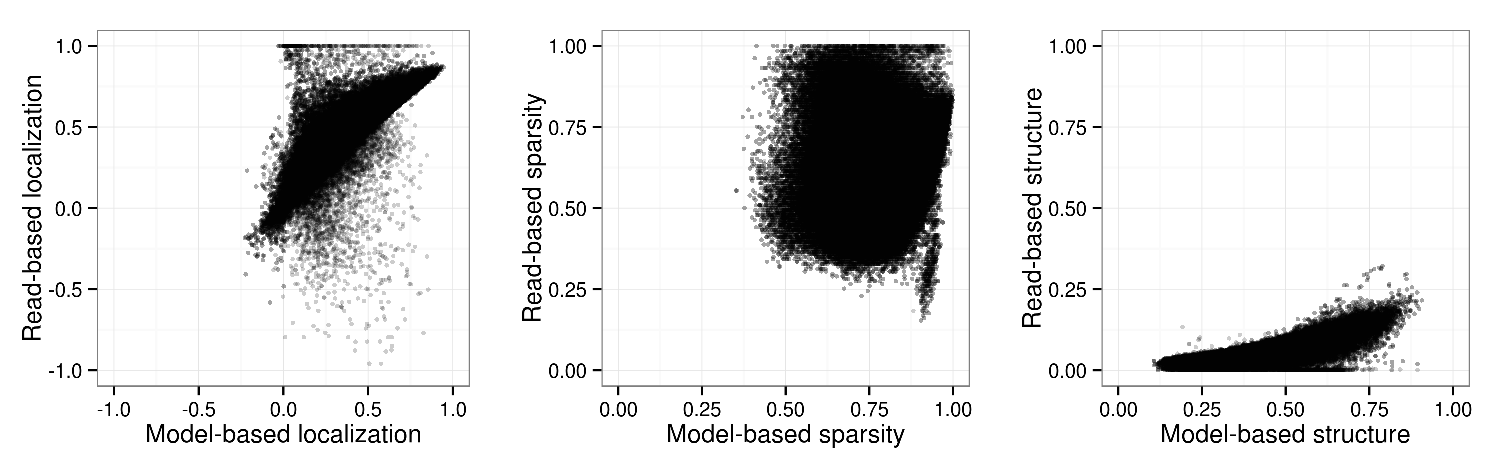
\includegraphics[width=0.95\textheight,angle=90]{figures/nucleosomes/figure_cluster_reproducibility_methods}
\caption{Joint distributions of of model-based and read-based estimates of cluster-level properties. \label{fig:methodComparison}}
\end{FPfigure}
\afterpage{\clearpage}

\subsection{Power analysis---cluster locations}
\label{sec:cluster}

\begin{FPfigure}
\centering
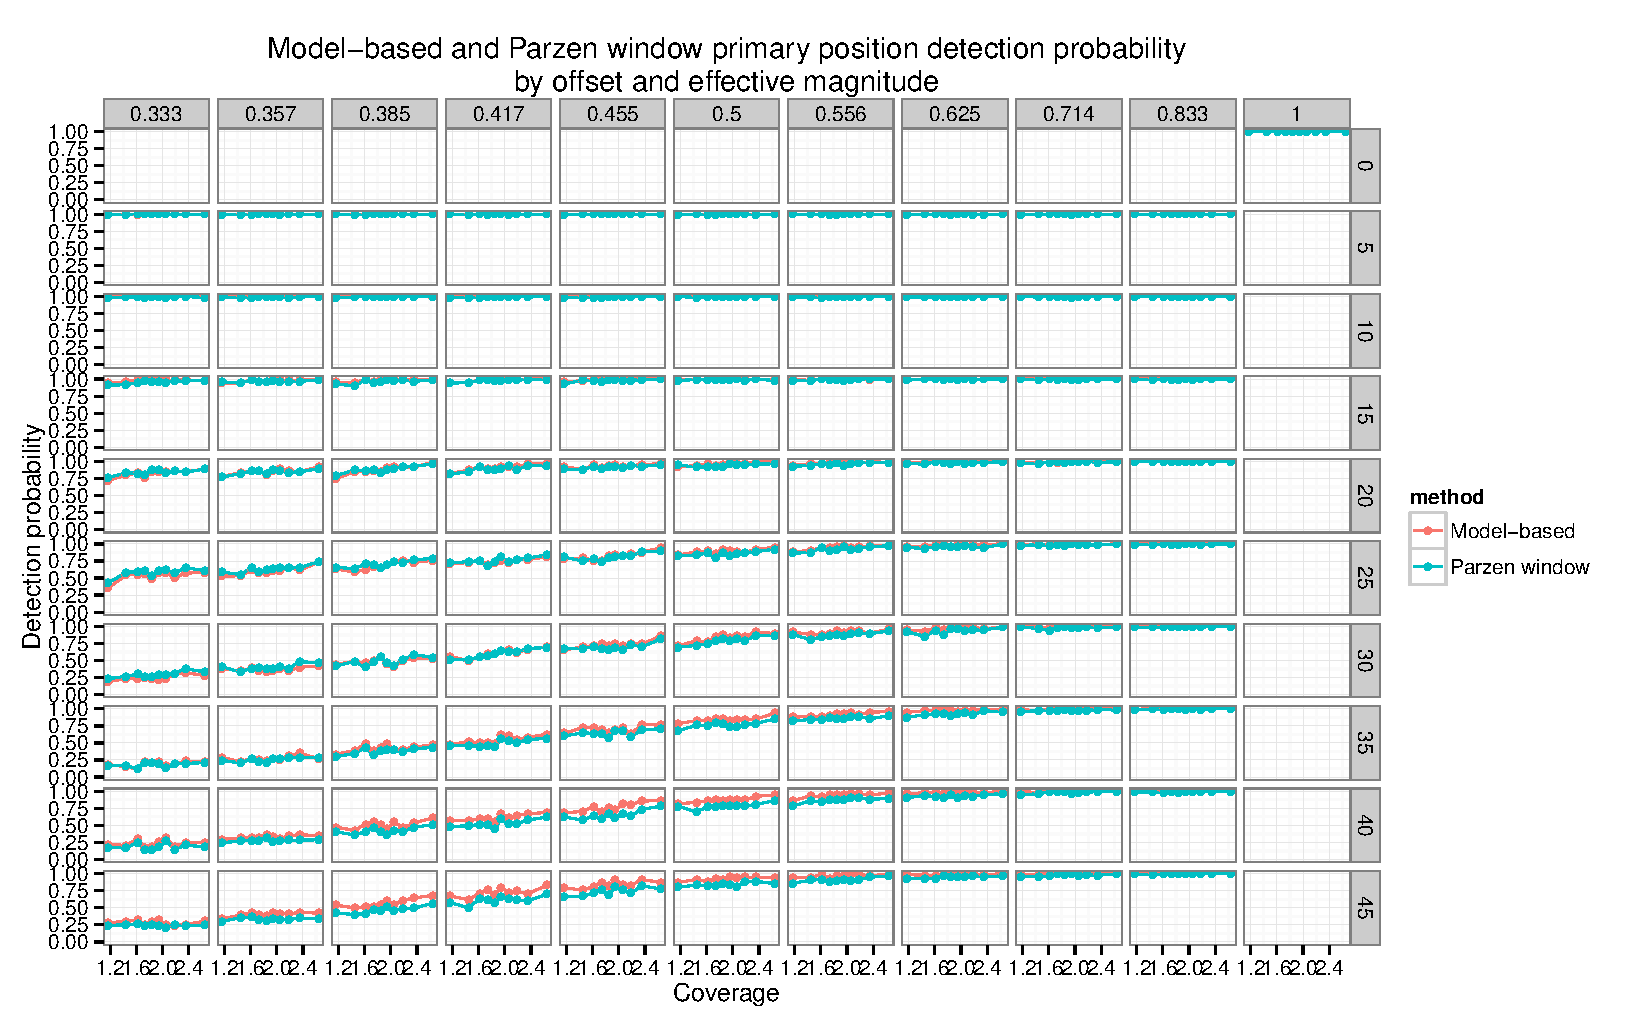
\includegraphics[page=1,width=0.95\textheight,angle=90]{figures/nucleosomes/plots_compare_power}
\caption{Power of model-based and Parzen window methods to detect cluster centers $\pm 5$bp vs. coverage by alternative position offset (rows) and effective magnitude of primary position (columns)}
\end{FPfigure}
\afterpage{\clearpage}

\begin{FPfigure}
\centering
\includegraphics[page=5,width=0.95\textheight,angle=90]{figures/nucleosomes/plots_compare_power}
\caption{Mean absolute position errors for model-based and Parzen window methods vs. coverage by alternative position offset (rows) and effective magnitude of primary position (columns)}
\end{FPfigure}
\afterpage{\clearpage}

\clearpage

\subsection{Power analysis---local concentrations}
\label{sec:detection}

\subsubsection{Primary positions}

\begin{FPfigure}
\centering
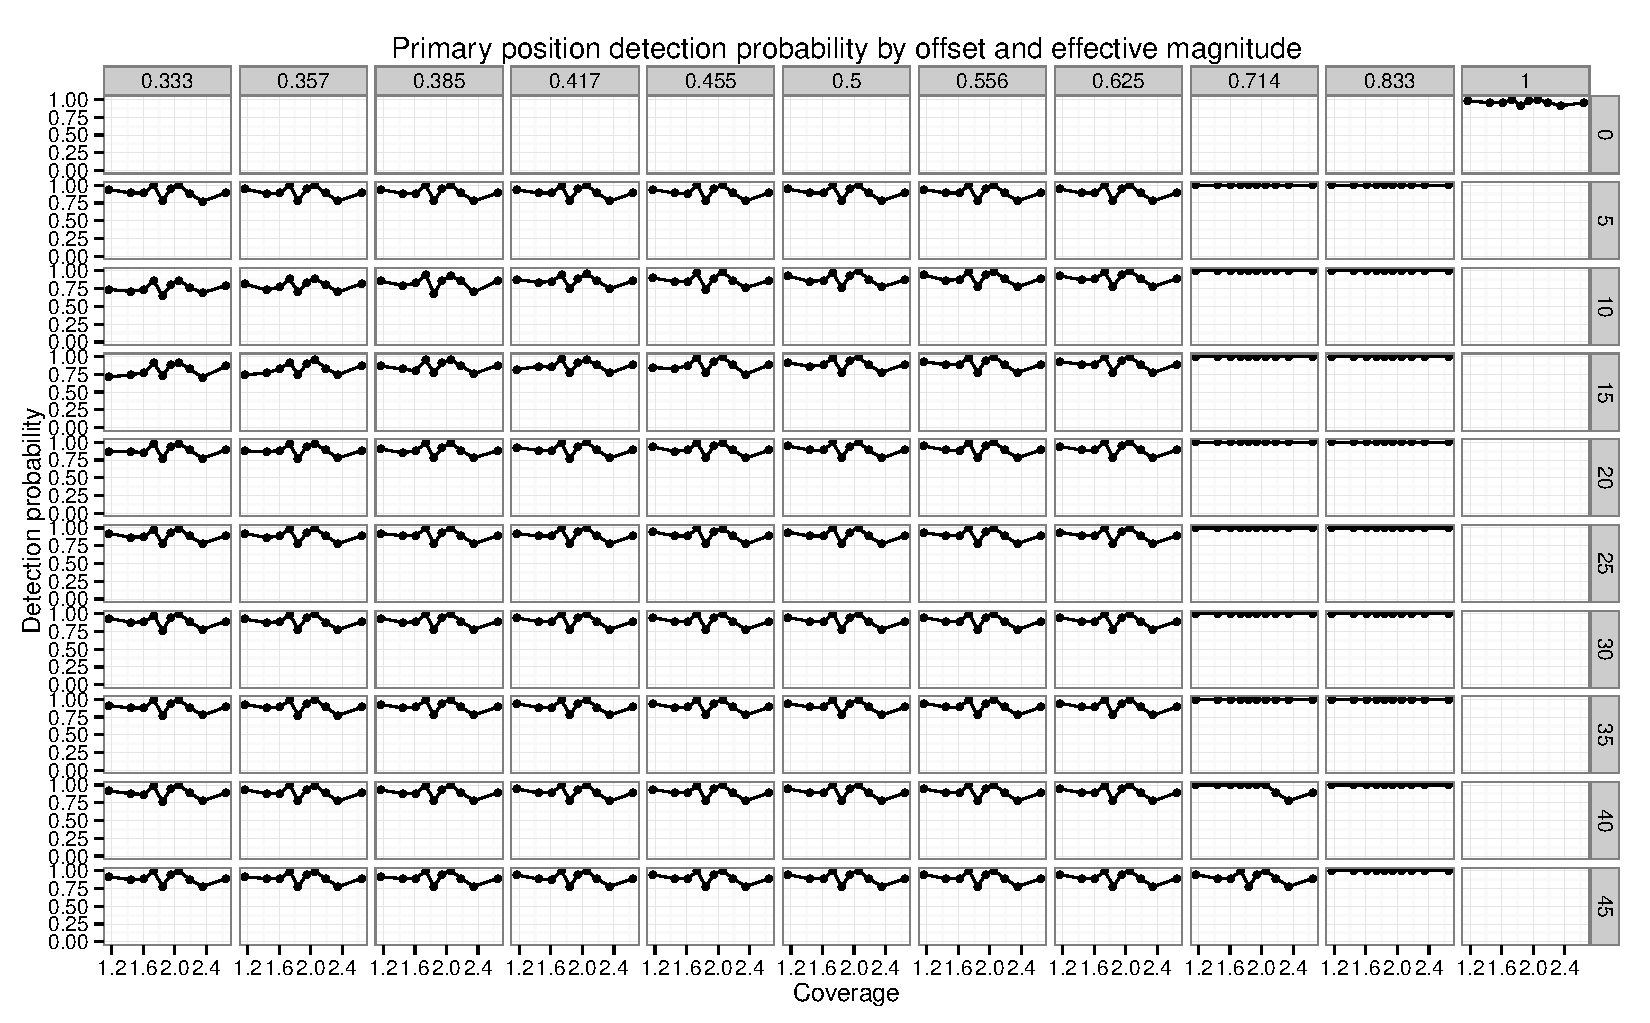
\includegraphics[page=1,width=0.95\textheight,angle=90]{figures/nucleosomes/plots_power_pm3}
\caption{Power of model-based method to detect individual primary positions $\pm 5$bp vs. coverage by alternative position offset (rows) and effective magnitude of primary position (columns)}
\end{FPfigure}
\afterpage{\clearpage}

\begin{FPfigure}
\includegraphics[page=5,width=0.95\textheight,angle=90]{figures/nucleosomes/plots_power_pm3}
\caption{Mean absolute position errors of model-based method for individual primary positions vs. coverage by alternative position offset (rows) and effective magnitude of primary position (columns)}
\end{FPfigure}
\afterpage{\clearpage}
\clearpage


\subsubsection{Alternative positions}

\begin{FPfigure}
\includegraphics[page=9,width=0.95\textheight,angle=90]{figures/nucleosomes/plots_power_pm3}
\caption{Power of model-based method to detect individual alternative positions $\pm 5$bp vs. coverage by alternative position offset (rows) and effective magnitude of alternative position (columns)}
\end{FPfigure}
\afterpage{\clearpage}

\begin{FPfigure}
\includegraphics[page=13,width=0.95\textheight,angle=90]{figures/nucleosomes/plots_power_pm3}
\caption{Mean absolute position errors of model-based method for individual alternative positions vs. coverage by alternative position offset (rows) and effective magnitude of alternative position (columns)}
\end{FPfigure}
\afterpage{\clearpage}
